\documentclass[14pt]{extbook}
\usepackage{multicol, enumerate, enumitem, hyperref, color, soul, setspace, parskip, fancyhdr} %General Packages
\usepackage{amssymb, amsthm, amsmath, bbm, latexsym, units, mathtools} %Math Packages
\everymath{\displaystyle} %All math in Display Style
% Packages with additional options
\usepackage[headsep=0.5cm,headheight=12pt, left=1 in,right= 1 in,top= 1 in,bottom= 1 in]{geometry}
\usepackage[usenames,dvipsnames]{xcolor}
\usepackage{dashrule}  % Package to use the command below to create lines between items
\newcommand{\litem}[1]{\item#1\hspace*{-1cm}\rule{\textwidth}{0.4pt}}
\pagestyle{fancy}
\lhead{Progress Quiz 10}
\chead{}
\rhead{Version C}
\lfoot{6232-9639}
\cfoot{}
\rfoot{Fall 2020}
\begin{document}

\begin{enumerate}
\litem{
Determine the vertical asymptotes and holes in the rational function below.\[ f(x) = \frac{9x^{3} -9 x^{2} -25 x + 25}{9x^{2} +27 x + 20} \]\begin{enumerate}[label=\Alph*.]
\item \( \text{Vertical Asymptotes of } x = -1.333 \text{ and } x = -1.667 \text{ with no holes.} \)
\item \( \text{Vertical Asymptotes of } x = -1.333 \text{ and } x = 1.667 \text{ with a hole at } x = -1.667 \)
\item \( \text{Vertical Asymptote of } x = -1.333 \text{ and hole at } x = -1.667 \)
\item \( \text{Holes at } x = -1.333 \text{ and } x = -1.667 \text{ with no vertical asymptotes.} \)
\item \( \text{Vertical Asymptote of } x = 1.0 \text{ and hole at } x = -1.667 \)

\end{enumerate} }
\litem{
Determine the horizontal and/or oblique asymptotes in the rational function below.\[ f(x) = \frac{16x^{3} -24 x^{2} -7 x + 15}{4x^{2} -9 x -9} \]\begin{enumerate}[label=\Alph*.]
\item \( \text{Horizontal Asymptote of } y = 3.0 \text{ and Oblique Asymptote of } y = 4x + 3 \)
\item \( \text{Horizontal Asymptote of } y = 4.0 \text{ and Oblique Asymptote of } y = 4x + 3 \)
\item \( \text{Horizontal Asymptote of } y = 4.0  \)
\item \( \text{Horizontal Asymptote at } y = 3.0 \)
\item \( \text{Oblique Asymptote of } y = 4x + 3. \)

\end{enumerate} }
\litem{
Which of the following functions \textit{could} be the graph below?
\begin{center}
    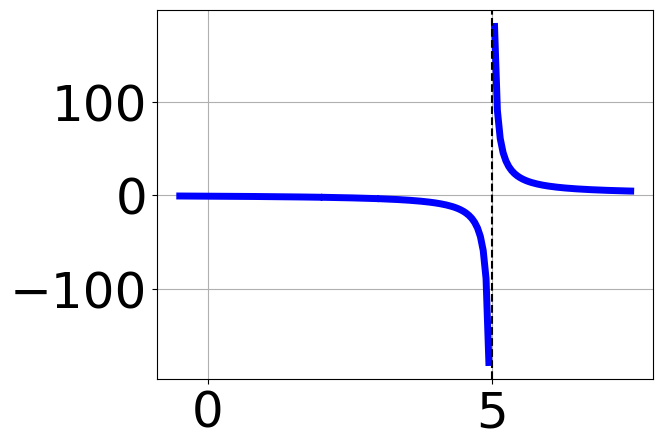
\includegraphics[width=0.5\textwidth]{../Figures/identifyGraphOfRationalFunctionC.png}
\end{center}
\begin{enumerate}[label=\Alph*.]
\item \( f(x)=\frac{x^{3} + x^{2} -14 x -24}{x^{3} +10 x^{2} +31 x + 30} \)
\item \( f(x)=\frac{x^{3} +4 x^{2} -x -4}{x^{3} -10 x^{2} +31 x -30} \)
\item \( f(x)=\frac{x^{3} + x^{2} -14 x -24}{x^{3} +10 x^{2} +31 x + 30} \)
\item \( f(x)=\frac{x^{3} -1 x^{2} -14 x + 24}{x^{3} -10 x^{2} +31 x -30} \)
\item \( \text{None of the above are possible equations for the graph.} \)

\end{enumerate} }
\litem{
Determine the vertical asymptotes and holes in the rational function below.\[ f(x) = \frac{12x^{3} +59 x^{2} +29 x -60}{8x^{2} +6 x -9} \]\begin{enumerate}[label=\Alph*.]
\item \( \text{Vertical Asymptotes of } x = -1.5 \text{ and } x = -1.667 \text{ with a hole at } x = 0.75 \)
\item \( \text{Vertical Asymptote of } x = -1.5 \text{ and hole at } x = 0.75 \)
\item \( \text{Vertical Asymptotes of } x = -1.5 \text{ and } x = 0.75 \text{ with no holes.} \)
\item \( \text{Holes at } x = -1.5 \text{ and } x = 0.75 \text{ with no vertical asymptotes.} \)
\item \( \text{Vertical Asymptote of } x = 1.5 \text{ and hole at } x = 0.75 \)

\end{enumerate} }
\litem{
Determine the horizontal and/or oblique asymptotes in the rational function below.\[ f(x) = \frac{12x^{3} -23 x^{2} -8 x + 12}{-20x^{3} -18 x^{2} +15 x -18} \]\begin{enumerate}[label=\Alph*.]
\item \( \text{None of the above} \)
\item \( \text{Vertical Asymptote of } y = 2  \)
\item \( \text{Horizontal Asymptote of } y = -0.600  \)
\item \( \text{Vertical Asymptote of } y = 0.600  \)
\item \( \text{Horizontal Asymptote of } y = 0  \)

\end{enumerate} }
\litem{
Which of the following functions \textit{could} be the graph below?
\begin{center}
    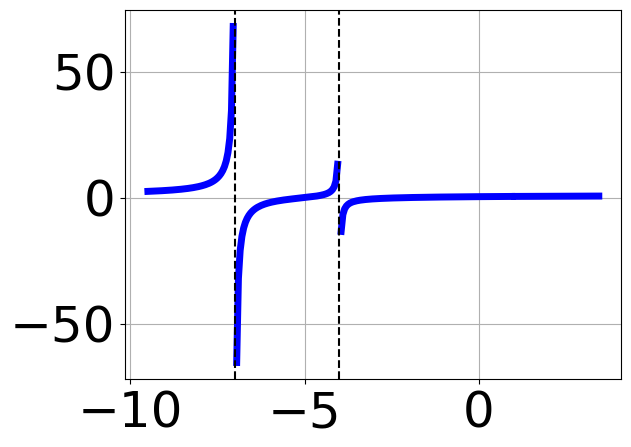
\includegraphics[width=0.5\textwidth]{../Figures/identifyGraphOfRationalFunctionCopyC.png}
\end{center}
\begin{enumerate}[label=\Alph*.]
\item \( f(x)=\frac{x^{3} -6 x^{2} +3 x + 10}{x^{3} -10 x^{2} +17 x + 28} \)
\item \( f(x)=\frac{x^{3} -6 x^{2} +3 x + 10}{x^{3} -10 x^{2} +17 x + 28} \)
\item \( f(x)=\frac{x^{3} +5 x^{2} -4 x -20}{x^{3} +10 x^{2} +17 x -28} \)
\item \( f(x)=\frac{x^{3} +6 x^{2} +3 x -10}{x^{3} +10 x^{2} +17 x -28} \)
\item \( \text{None of the above are possible equations for the graph.} \)

\end{enumerate} }
\litem{
Determine the horizontal and/or oblique asymptotes in the rational function below.\[ f(x) = \frac{12x^{3} -83 x^{2} +165 x -100}{4x^{2} +15 x -25} \]\begin{enumerate}[label=\Alph*.]
\item \( \text{Oblique Asymptote of } y = 3x -32. \)
\item \( \text{Horizontal Asymptote of } y = 3.0 \text{ and Oblique Asymptote of } y = 3x -32 \)
\item \( \text{Horizontal Asymptote of } y = -5.0 \text{ and Oblique Asymptote of } y = 3x -32 \)
\item \( \text{Horizontal Asymptote at } y = -5.0 \)
\item \( \text{Horizontal Asymptote of } y = 3.0  \)

\end{enumerate} }
\litem{
Determine the vertical asymptotes and holes in the rational function below.\[ f(x) = \frac{6x^{3} -41 x^{2} +89 x -60}{12x^{2} -25 x + 12} \]\begin{enumerate}[label=\Alph*.]
\item \( \text{Vertical Asymptote of } x = 0.5 \text{ and hole at } x = 1.333 \)
\item \( \text{Vertical Asymptotes of } x = 0.75 \text{ and } x = 1.333 \text{ with no holes.} \)
\item \( \text{Vertical Asymptotes of } x = 0.75 \text{ and } x = 2.5 \text{ with a hole at } x = 1.333 \)
\item \( \text{Vertical Asymptote of } x = 0.75 \text{ and hole at } x = 1.333 \)
\item \( \text{Holes at } x = 0.75 \text{ and } x = 1.333 \text{ with no vertical asymptotes.} \)

\end{enumerate} }
\litem{
Determine the horizontal and/or oblique asymptotes in the rational function below.\[ f(x) = \frac{5x^{2} -19 x + 12}{20x^{3} -51 x^{2} -47 x + 60} \]\begin{enumerate}[label=\Alph*.]
\item \( \text{Horizontal Asymptote of } y = 0.250 \text{ and Oblique Asymptote of } y = 4x + 5 \)
\item \( \text{Horizontal Asymptote at } y = 3.000 \)
\item \( \text{Horizontal Asymptote of } y = 0.250  \)
\item \( \text{Horizontal Asymptote of } y = 0 \)
\item \( \text{Oblique Asymptote of } y = 4x + 5. \)

\end{enumerate} }
\litem{
Determine the vertical asymptotes and holes in the rational function below.\[ f(x) = \frac{6x^{3} -17 x^{2} -3 x + 20}{8x^{2} -10 x -25} \]\begin{enumerate}[label=\Alph*.]
\item \( \text{Vertical Asymptotes of } x = -1.25 \text{ and } x = 2.5 \text{ with no holes.} \)
\item \( \text{Vertical Asymptote of } x = 0.75 \text{ and hole at } x = 2.5 \)
\item \( \text{Holes at } x = -1.25 \text{ and } x = 2.5 \text{ with no vertical asymptotes.} \)
\item \( \text{Vertical Asymptotes of } x = -1.25 \text{ and } x = 1.333 \text{ with a hole at } x = 2.5 \)
\item \( \text{Vertical Asymptote of } x = -1.25 \text{ and hole at } x = 2.5 \)

\end{enumerate} }
\end{enumerate}

\end{document}